\documentclass[11pt, oneside]{article}   	% use "amsart" instead of "article" for AMSLaTeX format
\usepackage{geometry}                		% See geometry.pdf to learn the layout options. There are lots.
\geometry{letterpaper}                   		% ... or a4paper or a5paper or ... 
%\geometry{landscape}                		% Activate for for rotated page geometry
%\usepackage[parfill]{parskip}    		% Activate to begin paragraphs with an empty line rather than an indent
\usepackage{graphicx}				% Use pdf, png, jpg, or eps§ with pdflatex; use eps in DVI mode
								% TeX will automatically convert eps --> pdf in pdflatex		
\usepackage{amssymb}

\title{CS 675 Course Project 3: Clock Synchronization}
\author{Zhonghua Xi}
%\date{}							% Activate to display a given date or no date

\begin{document}
\maketitle
%\section{}
%\subsection{}

\section{Design}
\subsection{Language Choice}
I choose python to implement the simple clock synchronization protocol. Mainly because python has native support for UDP socket programming, also python supports multiple platforms.
\subsection{Timeout Threshold}
Packet timeout threshold was set to 5 times of the average round trip time (10ms in current implementation) between client and server.
If a packet arrived after timeout, that packet will be dropped and regarded as a failure.
 
\section{Implementation}
Both client and server are implemented in python.

\subsection{Compile}
No compilation required.
\subsection{Run}
Start the server: \\
\$ ./server.py \\
Start the client: \\
\$ ./client.py server\_address


\section{Results}

\subsection{Setup}
Server: medusa-node1.vsnet.gmu.edu \\
Client: pearl.vsnet.gmu.edu (NTP turned off)\\
Running period: 24 hours

\subsection{Average Round Trip Time}
Average round trip time: 2.102ms

\subsection{Packet Loss Rate}
Request sent: 8533 \\
Response received: 8317 \\
Packet loss rate: 2.53 \%

\subsection{Average Clock Drift Rate}
Fit a linear model between {\it offset} and {\it elapsed time} \\ 
Average clock drift rate =  $-24.316 \times 10^{-6}s/s$

\begin{figure}[ht] %  figure placement: here, top, bottom, or page
   \centering
   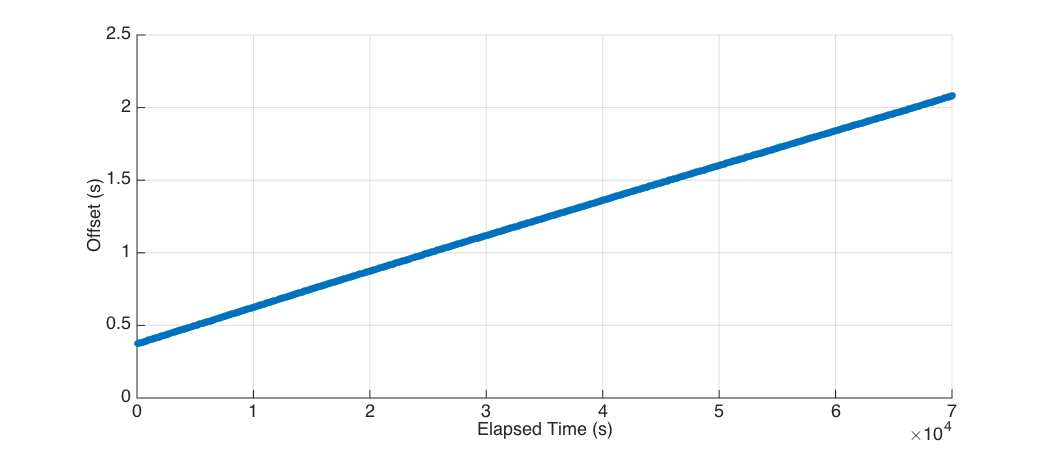
\includegraphics[width=6in]{../offset.png} 
   \caption{Scatter plot: Offset V.S. Elapsed Time.}
   \label{fig:cdr}
\end{figure}

\subsection{Histogram of Instantaneous Clock Drift Rate}
The shape is a mixture of gaussian distribution with one mean at $-25 \times 10^{-6} s/s$, one mean at $-42 \times 10^{-6} s/s$ and one mean at $-8 \times 10^{-6} s/s $. The middle is the main component which is the normal case with a normal distribution. The rest of two small components are due to server load and client load, context switch, thus the estimation of round trip and offset has a non-zero mean error.

\begin{figure}[ht] %  figure placement: here, top, bottom, or page
   \centering
   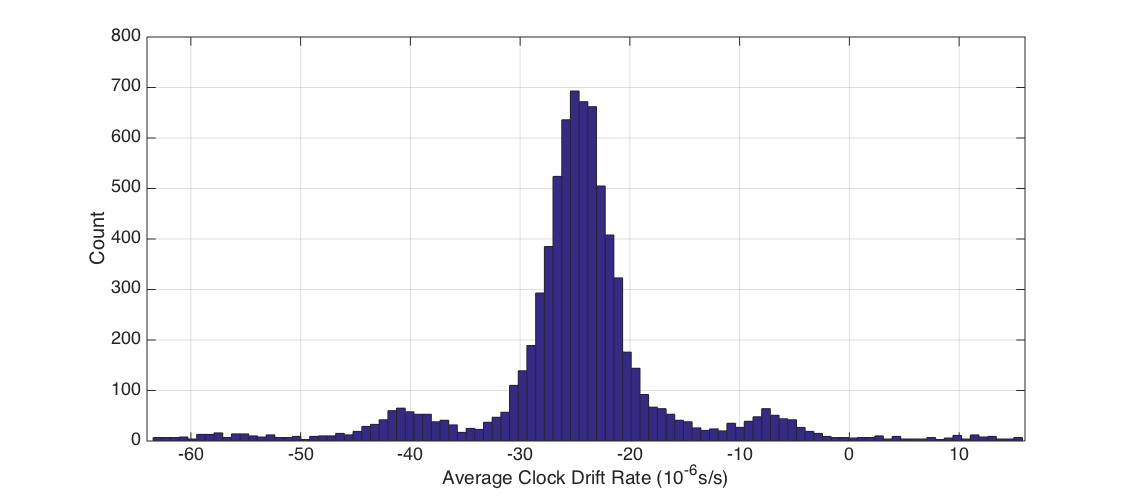
\includegraphics[width=6in]{../cdr.png} 
   \caption{Histogram of average clock drift rate.}
   \label{fig:cdr}
\end{figure}

\end{document}  